\documentclass[12pt]{article}

\usepackage{amsmath}
\usepackage{amssymb}
\usepackage{graphicx}

\counterwithin*{equation}{section}
\counterwithin*{equation}{subsection}
\addtolength\parskip{\bigskipamount}

\graphicspath{ {./images/} } 

\begin{document}
\section{Cylindrical Coordinates}

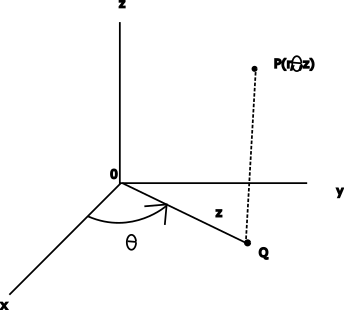
\includegraphics{cylindricalcoordinate}\\%
\underline{Cylindrical to rectangular:}\\%
$x=r\cos\theta$\\%
$y=r\sin\theta$\\%
$z=z$

\subsection{Cylindrical Coordinates Example 2}
Find the cylindrical coordinates for:\\%
$Q(x,y,z) = Q(2,-2,3)$
\begin{align}
	r^2=x^2+y^2=4+4=8\\%
	r=+-2\sqrt{2}\\%
	\tan\theta=\frac{y}{x}=\frac{-2}{2}=-2 \Rightarrow \theta =- \frac{\pi}{4}+\pi n
\end{align}

\subsection{Cylindrical Coordinates Example 3}
\underline{Sketch}\\%
a) $\theta=\frac{\pi}{4}$\\%
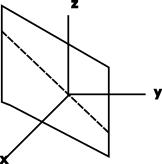
\includegraphics{planecylindrical}\\%
b) $r=2$\\%
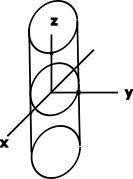
\includegraphics{cylinderpolar}\\%
c) $z=r$\\%
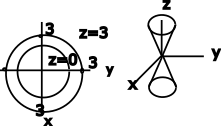
\includegraphics{conepolar}
\subsection{Cylindrical Coordinates Example 4}
Consider $x^2+y^2-z^2=1$\\%
a) Classify this quadric surface\\%
Hyperboloid of \underline{one} sheet\\%
b) Find a cylindrical equation for this surface\\%
$x^2+y^2=r^2$\\%
$r^2-z^2=1$\\%
$r^2=z^2+1$

\section{Spherical Coordinates}	
$(,\theta,\phi)$\\%
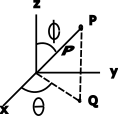
\includegraphics{sphericalcoordinate}
\subsection{Spherical Coordinates Example 1}
Convert $P(2,\frac{\pi}{3},\frac{\pi}{4})$ From spherical to rectangular coordinate

\subsection{Spherical Coordinates Example 2}
Convert $Q(2\sqrt{3},0,-2)$ from rectangular to spherical coordinates.

\subsection{Spherical Coordinates Example 3}
Find a spherical coordinates equation for the given rectangular equation.\\%
$x^2+y^2-z^2=1$, hyperboloid of one sheet\\%
hi
\subsection{Spherical Coordinates Example 4}
Find a rectangular coordinates equation for the given spherical equation. If possible, identify the object.\\%
a)roe = 1\\%
b)roe $= 2\cos\theta\sin\phi$\\%
c)(roe)$\sin\phi=2$

\end{document}
